\documentclass[15pt]{beamer}

\usepackage[utf8]{inputenc}
\usepackage[english]{babel}
\usepackage{amsmath}
\usepackage{natbib}
\usepackage{tikz}
\usepackage{amsfonts}
\usepackage{amssymb}
\usepackage{polski}
\usepackage{amsthm}
\usepackage{wrapfig}
\usepackage{ amssymb }
\usepackage{ dsfont }
\usepackage{ fontawesome }
\usepackage{ bclogo}

\newtheorem{hypothesis}[theorem]{Hipoteza}

\useoutertheme{infolines}
\setbeamertemplate{note page}[plain]
\DeclareFixedFont{\ttb}{T1}{txtt}{bx}{n}{12} % for bold
\DeclareFixedFont{\ttm}{T1}{txtt}{m}{n}{12}  % for normal
\usepackage{color}
\definecolor{deepblue}{rgb}{0,0,0.5}
\definecolor{deepred}{rgb}{0.6,0,0}
\definecolor{deepgreen}{rgb}{0,0.5,0}

% === Minimal beamer === %
\setbeamertemplate{frametitle}
  {\begin{centering}\smallskip
   \insertframetitle\par
   \smallskip\end{centering}
   }

% Define some colors:
\definecolor{DarkFern}{HTML}{407428}
\definecolor{DarkCharcoal}{HTML}{4D4944}
\colorlet{Fern}{DarkFern!85!white}
\colorlet{Charcoal}{DarkCharcoal!85!white}
\colorlet{LightCharcoal}{Charcoal!50!white}
\colorlet{AlertColor}{orange!80!black}
\colorlet{DarkRed}{red!70!black}
\colorlet{AlertColor}{red!70!black}
\colorlet{DarkBlue}{blue!70!black}
\colorlet{DarkGreen}{green!70!black}

\setbeamertemplate{navigation symbols}{}
\setbeamertemplate{footline}{}

% Use the colors:
\setbeamercolor{title}{fg=DarkRed}
\setbeamercolor{frametitle}{fg=DarkRed}
\setbeamercolor{normal text}{fg=Charcoal}
\setbeamercolor{block title}{fg=black,bg=Fern!25!white}
\setbeamercolor{block body}{fg=black,bg=Fern!25!white}
\setbeamercolor{alerted text}{fg=AlertColor}
\setbeamercolor{itemize item}{fg=Charcoal}

\usetikzlibrary{shapes.misc}

\tikzset{cross/.style={cross out, draw=black, minimum size=2*(#1-\pgflinewidth), inner sep=0pt, outer sep=0pt},
%default radius will be 1pt. 
cross/.default={1pt}}

\usebackgroundtemplate{
\begin{tikzpicture}[remember picture, overlay]
  \node [above=0.37cm, left=1.0cm] at (current page.south east)
     {  
     
\includegraphics[width=0.15\paperwidth,height=0.15\paperheight,keepaspectratio]{fig/gmum.jpg}
     };
     \node [above=0.31cm, left=0.1cm] at (current page.south east){
    \insertframenumber/\inserttotalframenumber     
     };  
\end{tikzpicture}
}

\title[ICLR zapłata]{Selected ICLR 2017 Papers}
\author{Agnieszka Pocha}
\institute{Jagiellonian University}
\date{19.05.2017, Kraków}

\begin{document}

\begin{frame}
  \titlepage
\end{frame}

% Uncomment these lines for an automatically generated outline.
% \begin{frame}{Outline}
%  \tableofcontents
% \end{frame}

% \section{Designing Neural Network Architectures using Reinforcement Learning}


\begin{frame}{Designing Neural Network Architectures using Reinforcement Learning}
  Bowen Baker, Otkrist Gupta, Nikhil Naik, Ramesh Raskar

  \vspace{0.05in}

  \begin{block}{Abstract}
  Designing NN architectures is slow and laborious. We would like to have an automatic and successful method to do it for us.\vspace{0.04in}
  Authors introduce MetaQNN - a \textbf{reinforcement learning method} based on \textbf{Q-learnig} algorithm that finds highly performing architectures.\vspace{0.05in}
  Their models:
  \begin{itemize}
  \item beat on CIFAR, MNIST \& SVHN best performing models that share similar architecture
  \item compare well with state-of-the-art models
  \item are suitable for transfer learning
  \end{itemize}
  Moreover, authors show that their method is stable.

  \end{block}
\end{frame}


\begin{frame}{Shortly}
\centering 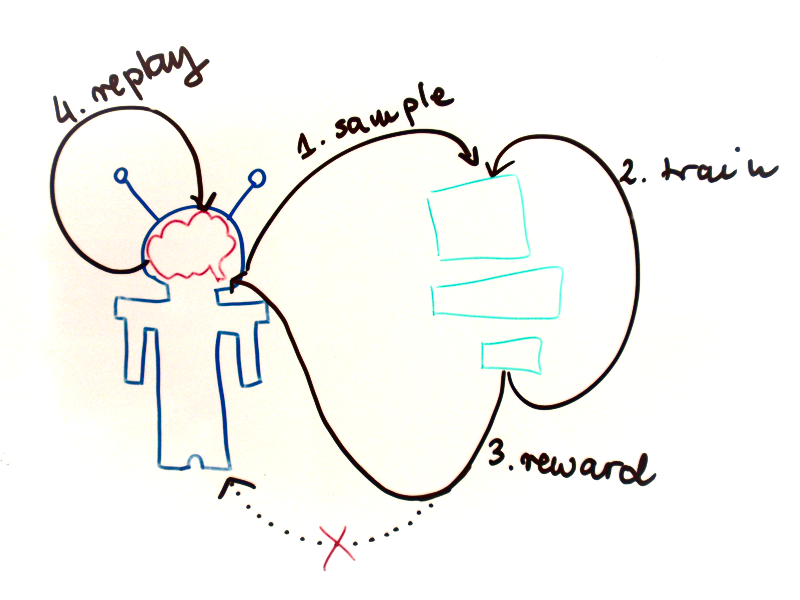
\includegraphics[width=0.7\textwidth]{model.png}

\raggedright
  Learning agent sequentially chooses CNN layers using \textbf{Q-learnig} with an \textbf{$\epsilon$-greedy exploration strategy} and \textbf{experience replay}.
\end{frame}


\begin{frame}{$\epsilon$-greedy exploration strategy}
  Choose what you think is the best option with probability $1-\epsilon$ and choose a random action with probability $\epsilon$.

  \begin{center}
  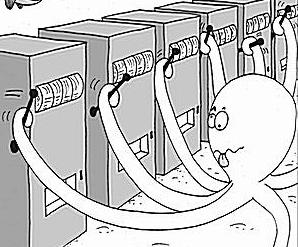
\includegraphics[width=0.6\textwidth]{exploration.jpg}
  \end{center}

  \begin{center}
  \begin{tiny}
  \url{http://research.microsoft.com/en-us/projects/bandits/}  
  \end{tiny}
  \end{center}
\end{frame}


\begin{frame}{Q-learnig}
  Let $\mathcal{S}$ - state space, $\mathcal{U}$- action space, $\mathcal{U}(s_i) \in \mathcal{U}$ - actions possible while in state $s_i$.
  \vskip0.1in
  In an environment with stochastic transitions, an agent in state $s_i$ taking some action $u \in \mathcal{U}$ will \textbf{transition} to state $s_j$ with probability $p_{s'|s, u}(s_j | s_i, u)$ which may be unknown to the agent.
  \vskip0.1in
  At each timestep $t$, the agent is given a \textbf{reward} $r_t$, dependent on the transition from state $s$ to $s'$ and action $u$. The reward may also be stochastic according to a distribution $p_{r|s', s, u}$.
  \vskip0.1in
  The agent's \textbf{goal} is to maximize the \textbf{total expected reward} over all possible trajectories, i.e. $max_{\tau_i \in \tau R_{\tau_i}}$, where the total expected reward for a trajectory $\tau_i$ is

  \begin{center}
  $R_{\tau_i} = \Sigma_{(s, u, s') \in \tau_i} \mathds{E}_{r|s, u, s'}[r|s, u, s']$
  \end{center}
\end{frame}


\begin{frame}{Q-learnig}
  Let $\mathcal{S}$ - state space, $\mathcal{U}$- action space, $\mathcal{U}(s_i) \in \mathcal{U}$ - actions possible while in state $s$.

  \begin{center}
  $R_{\tau_i} = \Sigma_{(s, u, s') \in \tau_i} \mathds{E}_{r|s, u, s'}[r|s, u, s']$
  \end{center}

  The number of possible trajectories makes the problem untractable, therefore we define the maximization problem recursively in terms of subproblems as follows: for any state $s_i \in S$ and subsequent action $u \in \mathcal{U}(s_i)$, we define the \textbf{maximum total expected reward} to be $Q^*(s_i, u)$. The recursive maximization equation, which is known as \textbf{Bellman's Equation}, can be written as:

  \begin{center}
  $Q^*(s_i, u) = \mathds{E}_{s_j|s_i, u}[ \mathds{E}_{r|s_i, u, s_j}[r|s_i, u, s_j] + \gamma max_{u' \in \mathcal{U}(s_j)} Q^*(s_j, u') ]$ 
  \end{center}

  We usually cannot solve it analytically but we can define an \textbf{iterative update}.
\end{frame}


\begin{frame}{Q-learning}
  \begin{itemize}
  \item \textbf{model-free}
  \item \textbf{off-policy}
  \item two parameters:
  \begin{itemize}
  \item $\alpha$ - \textbf{learning rate}
  \item $\lambda$ - \textbf{discount factor} (weight given to short term rewards over future rewards)
  \end{itemize}
  \end{itemize}
  
  Here:
  \begin{itemize}
  \item \textbf{action} - choosing next layer along with its parameters (size, stride...)
  \item \textbf{state} - the current state of the network topology
  \item \textbf{reward} - performance on validation set (5K samples, with unchanged class distribution)
  \end{itemize}
\end{frame}


\begin{frame}{Experience replay}
  Use single experience multiple times for an iterative update.
  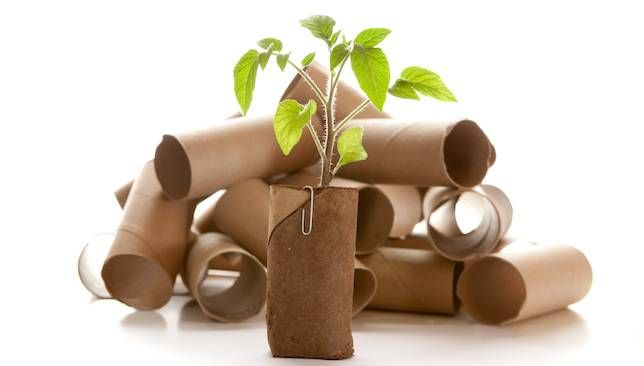
\includegraphics[width=0.9\textwidth]{reuse.jpg}\\
  \begin{tiny}
  \url{https://www.shutterstock.com/image-photo/empty-toilet-paper-roll-recycled-seedling-134967662?src=ijY4nrNlx43dUDT2n_Cjsw-1-4}
  \end{tiny}
\end{frame}


\begin{frame}{Shortly (again)}
  \centering
  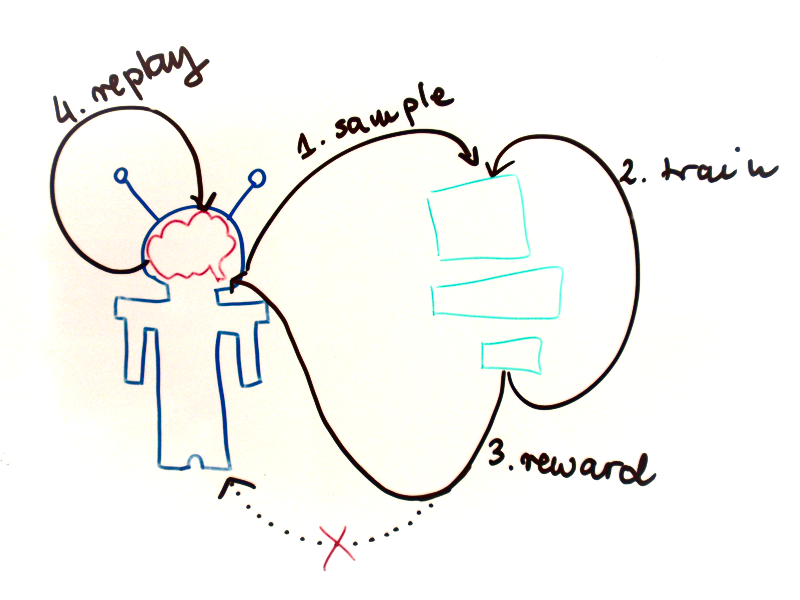
\includegraphics[width=0.7\textwidth]{model.png}

  \raggedright
  Learning agent sequentially chooses CNN layers using \textbf{Q-learnig} with an \textbf{$\epsilon$-greedy exploration strategy} and \textbf{experience replay}.
\end{frame}


\begin{frame}{Training models}
  Models were trained in an aggresive fashion (stop this violence!) what made the process less costly.
  \begin{itemize}
  \item dropout every 2 layers
  \item 20 epochs
  \item Adam
  \item batch size 128
  \item learning rate 0.001 reduced by a factor of 0.2 every 5 epochs
  \item Xavier initialization (Glorot \& Bengio 2010)
  \end{itemize}

  \textbf{Time:} 8-10 days for each dataset on 10 NVIDIA GPUs (GMUM needs more GPUs).
\end{frame}


\begin{frame}{Again same picture but now we should understand it completely}
  \centering
  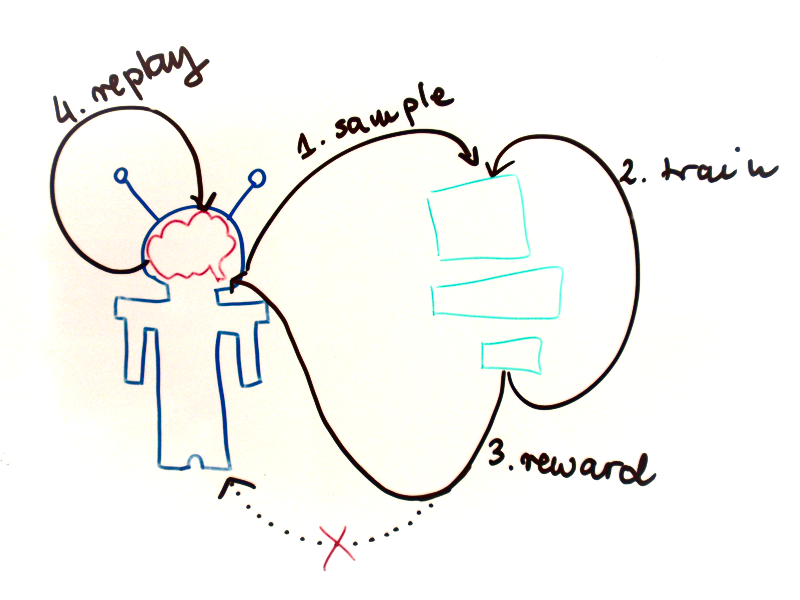
\includegraphics[width=0.65\textwidth]{model.png}  
  
  \raggedright
  Learning agent sequentially chooses CNN layers using \textbf{Q-learnig} with an \textbf{$\epsilon$-greedy exploration strategy} and \textbf{experience replay}.
\end{frame}

\begin{frame}{Experiments}
It grows! It means that the architectures chosen greedily/later (exploitation) are better than those randomly sampled (exploration) - the agent has learned something.
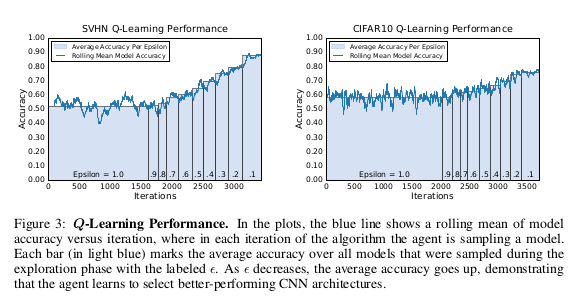
\includegraphics[width=0.88\textwidth]{experiments.png}
\end{frame}

\begin{frame}{Experiments}
It learns! It means that the architectures chosen greedily/later (exploitation) are better than those randomly sampled (exploration) - the agent has learned something.
\begin{center}
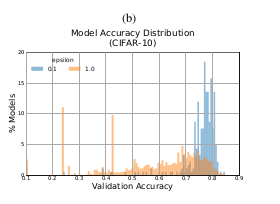
\includegraphics[width=0.63\textwidth]{exp2.png}
\end{center}
\end{frame}

\begin{frame}{Results}
After short training all those architectures 10 best were chosen and well tuned. Finally, 5 best were chosen to become ensemble.
\vskip0.1in
\begin{itemize}
  \item beat on CIFAR, MNIST \& SVHN best performing models that share similar architecture
  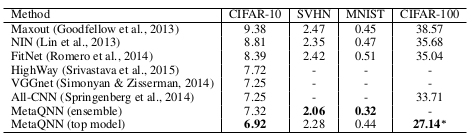
\includegraphics[width=0.8\textwidth]{best_on_similar.png}
  \end{itemize}
\end{frame}

\begin{frame}{Results}
  \begin{itemize}
  \item compare well with state-of-the-art models
  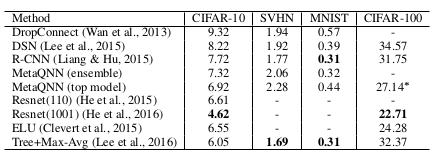
\includegraphics[width=0.86\textwidth]{state_art.png}
  \item are suitable for transfer learning
  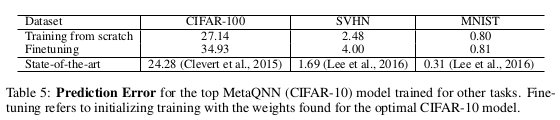
\includegraphics[width=0.85\textwidth]{transfer.png}
  \end{itemize}
\end{frame}

\begin{frame}{Results}
  \begin{itemize}
  \item stability
  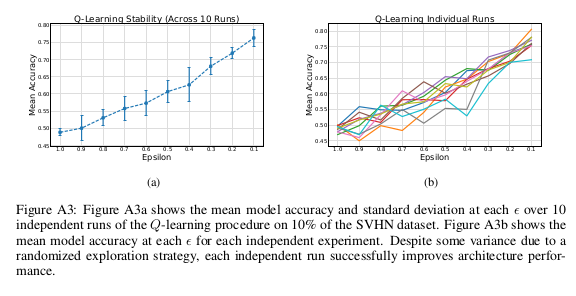
\includegraphics[width=0.9\textwidth]{stability.png}
  \end{itemize}
\end{frame}


\begin{frame}{My problem with this paper}
  \centering
  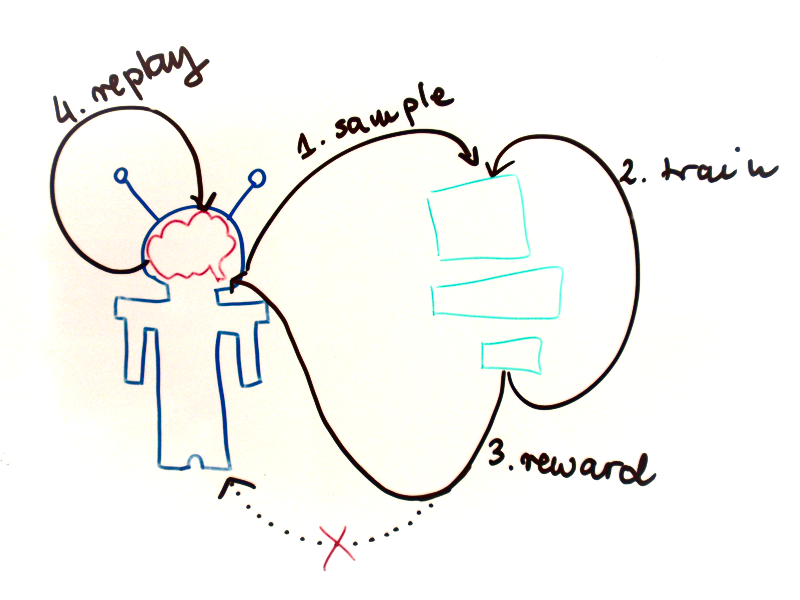
\includegraphics[width=0.7\textwidth]{model.png}
  
  \raggedright
  Late architectures (best performing) might not be chosen for replay i.e. not used for  training at all while early architectures (randomly performing) will be overrepresented.
\end{frame}

\begin{frame}{My problem with this paper}
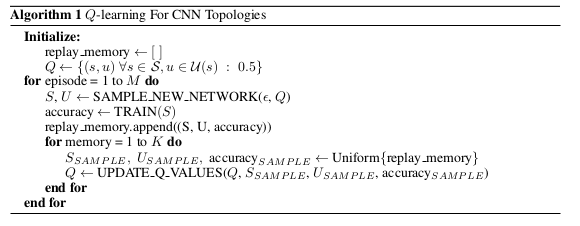
\includegraphics[width=\textwidth]{algorithm-1.png}

Late architectures (best performing) might not be chosen for replay i.e. not used for training at all, while early architectures (randomly performing) will be overrepresented.

\vskip0.1in
\begin{center}
\textbf{WHY?}
\end{center}
\end{frame}


\begin{frame}{Important note}
  \begin{center}
  \Huge{\faLightbulbO}
\end{center}

"While we report results for image classification problems, our method could be applied to different problem settings, including supervised (e.g., classification, regression) and unsupervised (e.g., autoencoders)"
\end{frame}


\begin{frame}{More}
  \centering
  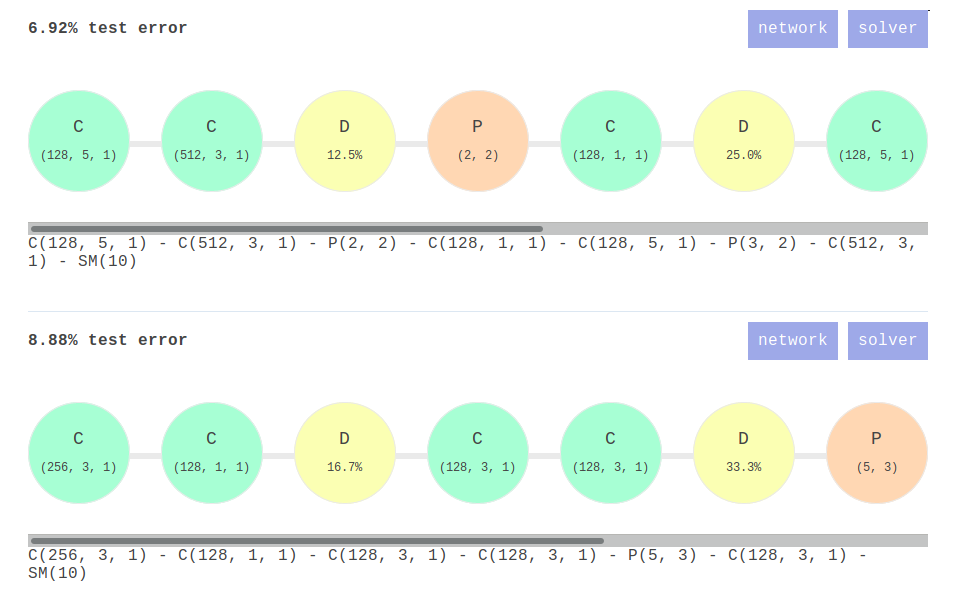
\includegraphics[width=0.8\textwidth]{bowen.png}

  \begin{itemize}
  \item arXiv 1611.02167 \url{https://arxiv.org/abs/1611.02167}
  \item GitHub \url{https://bowenbaker.github.io/metaqnn/}
  \end{itemize}
\end{frame}

% \section{Adversarial Examples in the Physical World}


\begin{frame}{Adversarial Examples in the Physical World}
  Alexey Kurakin, Ian J. Goodfellow, Samy Bengio

  \vspace{0.1in}

  \begin{block}{Abstract}
  An adversarial example is a sample of input data which has been modified very slightly in a way that is intended to cause a machine learning classifier to missclassify it. Adversarial examples pose security concerns because they could be used to perform attack on machine learning systems.
  \vskip0.1in
  \begin{enumerate}
  \item Authors found that a large fraction of adversarial examples generated for the original model remain missclassified even when perceived through a camera or altered with another transformation.
  \item They also demonstrated that the physical adversarial sample constructed for one model would fool another model.
  \end{enumerate}
  
  \end{block}
\end{frame}


\begin{frame}{Adversarial Examples}
  \begin{center}
  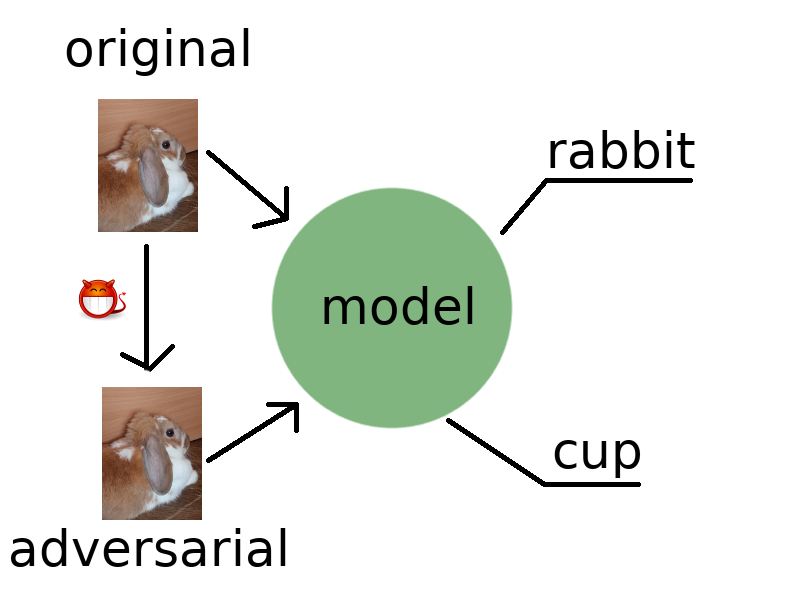
\includegraphics[width=0.75\linewidth]{adversarial.png}
  \end{center}
\end{frame}


\begin{frame}{Setup}
  \begin{center}
  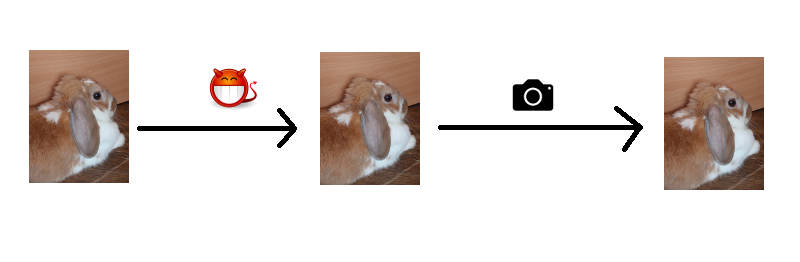
\includegraphics[width=0.9\linewidth]{photo.png}
  \vskip0.1in
  \begin{huge}
  \bcquestion
  \end{huge}
  \end{center}
\end{frame}


\begin{frame}{Actual outcome}
  \begin{center}
  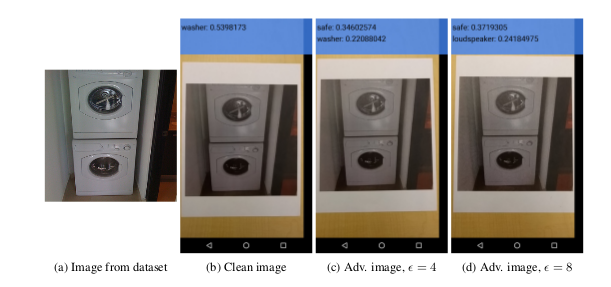
\includegraphics[width=\linewidth]{washer.png}
  \end{center}
\end{frame}

\begin{frame}{Methods for generating adversarial examples}
 \begin{itemize}
 \item \textbf{Fast method}
 \vskip0.1in
 \begin{center}
 $\textbf{X}^{adv} = \textbf{X} + \epsilon sign(\nabla_XJ(\textbf{X}, y_{true}))$
 \end{center}
 \item \textbf{Basic iterative method}
 \vskip0.1in
 \begin{center}
 $\textbf{X}^{adv}_0 = \textbf{X}, \textbf{X}^{adv}_{N+1} = Clip_{X, \epsilon}\{\textbf{X}^{adv}_N + \alpha sign(\nabla_XJ(\textbf{X}^{adv}_N, y_{true}))\}$
 \end{center}
 \item \textbf{Iterative least-likely class method}
 \vskip0.1in
 \begin{center}
 $\textbf{X}^{adv}_0 = \textbf{X}, \textbf{X}^{adv}_{N+1} = Clip_{X, \epsilon}\{\textbf{X}^{adv}_N - \alpha sign(\nabla_XJ(\textbf{X}^{adv}_N, y_{LL}))\}$
 \end{center}
 \end{itemize}

  \vskip0.1in
  where $J(\cdot, \cdot)$ is a cross-entropy cost function of the neural network, $Clip_{X, \epsilon}\{\textbf{X}'\}$ is a function which performs per-pixel clipping of the image $\textbf{X}'$ so that the result will be in the neighbourhood of the source image $\textbf{X}$, $y_{LL}$ is the least likely class.
\end{frame}

\begin{frame}{Methods for generating adversarial examples}
  \centering
  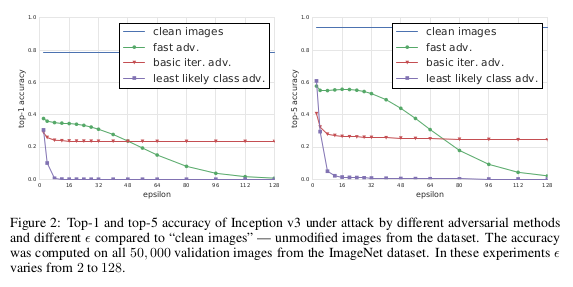
\includegraphics[width=\linewidth]{fig2.png}
  
  \raggedright
  None of these methods guarantees that generated image will be misclassified.
\end{frame}

\begin{frame}{What is the difference between those methods?}
  \begin{center}
  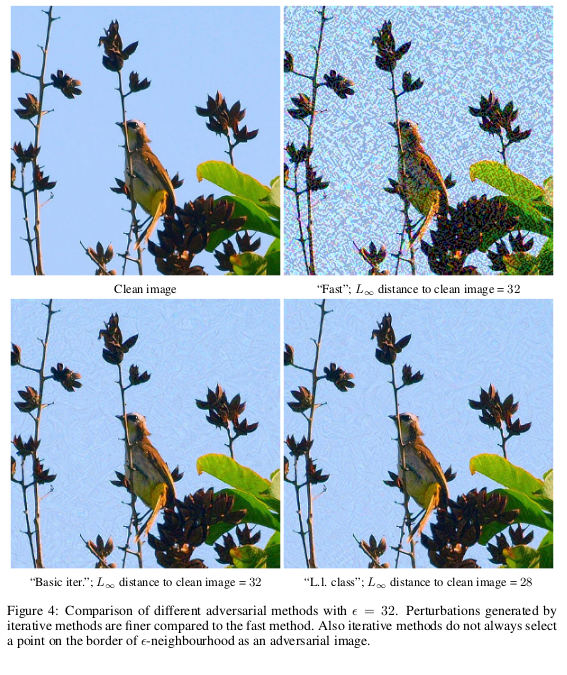
\includegraphics[width=0.55\linewidth]{different_methods.png}
  \end{center}
\end{frame}

\begin{frame}{Okay, but what doeas it mean: epsilon = 32?}
  \begin{center}
  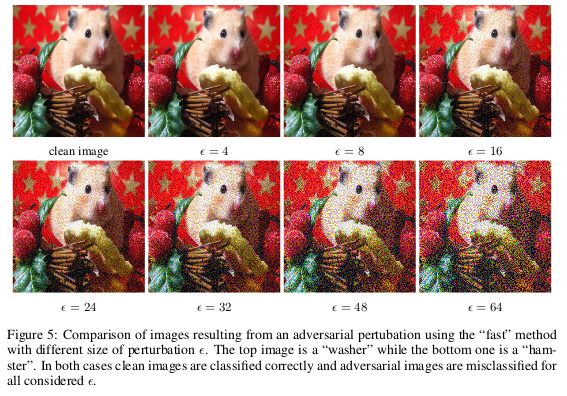
\includegraphics[width=0.8\linewidth]{epsilon.png}
  \end{center}
\end{frame}


\begin{frame}{Experiments}
  \textbf{Destruction rate}
  \vskip0.1in
  Let $n$ be number of images used to compute the destruction rate, $\textbf{X}^k$ an image from dataset, $y^k_{true}$ - true class of $k-th$ image, $\textbf{X}^k_{adv}$ - the corresponding adversarial image, $T(\cdot)$ - an arbitrary image transformation, $C(\textbf{X}, y)$ - an indicator function:

  \begin{center}
  $C(\textbf{X}, y) = \begin{cases} \displaystyle {1} & \mbox{if image \textbf{X} is classified as y}, \\[2ex] \displaystyle {0}& \mbox{otherwise } , \end{cases}$
  \end{center}

  Then, the destruction rate is defined as:

  \begin{center}
  $d = \frac{\sum^n_{k=1}C(\textbf{X}^k, y^k_{true})\overline{C(\textbf{X}^k_{adv}, y^k_{true})}C(T(\textbf{X}^k_{adv}),  y^k_{true})}{\sum^n_{k=1}C(\textbf{X}^k, y^k_{true})\overline{C(\textbf{X}^k_{adv}, y^k_{true})}}$
  \end{center}

  where $\overline{C(\textbf{X}, y)}$ is a binary negation.
\end{frame}


\begin{frame}{Experiments}
\textbf{Average case} - images used to calculate measures were chosen randomly.
\vskip0.1in
\textbf{Prefiltered case} (aggresive attack (stop this violence!)) - images used to calculate measures were chosen in such a way that all clean images were classified correctly and all adversarial images were classified incorrectly.
\end{frame}


\begin{frame}{Results}
  \begin{enumerate}
  \item Authors found that a large fraction of adversarial examples generated for the original model remain missclassified even when perceived through a camera or altered with another transformation.
  \item They also demonstrated that the physical adversarial sample constructed for one model would fool another model.
  \end{enumerate}
\end{frame}

\begin{frame}{Results}
  \begin{center}
  \textbf{Average case accuracy}
  \vskip0.1in
  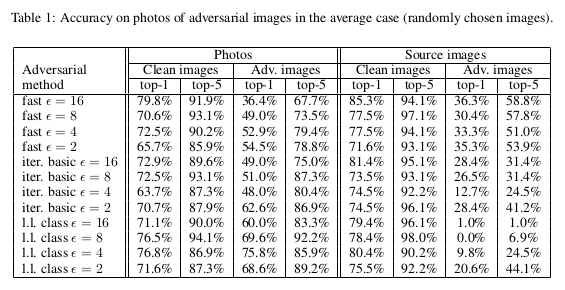
\includegraphics[width=\linewidth]{tab1.png}
  \end{center}
\end{frame}


\begin{frame}{Results}
  \begin{center}
  \textbf{Prefiltered case accuracy}
  \vskip0.1in
  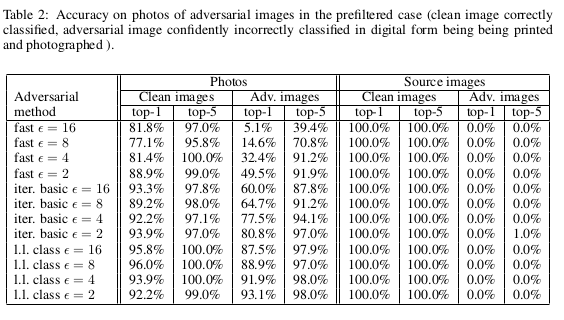
\includegraphics[width=0.9\linewidth]{tab2.png}
  \end{center}
\end{frame}


\begin{frame}{Results}
  \begin{center}
  \textbf{Destruction rate}
  \vskip0.1in
  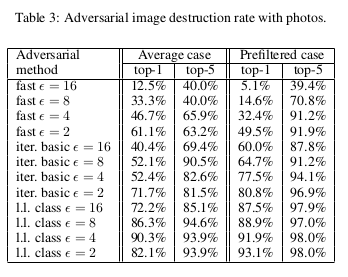
\includegraphics[width=0.65\linewidth]{tab3.png}
  \end{center}
\end{frame}


\begin{frame}{What about other transformations?}
  \begin{center}
  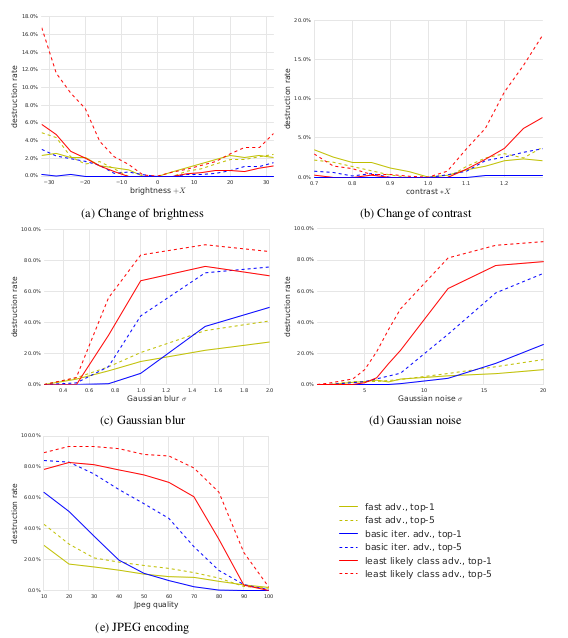
\includegraphics[width=0.55\linewidth]{other_transformations.png}
  \end{center}
\end{frame}


\begin{frame}{Adversarial examples transfer}
  \begin{center}
  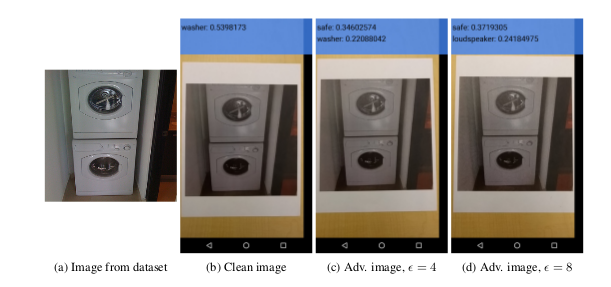
\includegraphics[width=0.9\linewidth]{washer.png}
  \end{center}
  
  Adversarial exmaples constructed for pre-trained ImageNet Inception classifier (Szegedy et. al, 2015) fool the TensorFlow camera demo.
\end{frame}


\begin{frame}{More}
  \begin{itemize}
  \item arXiv 1607.02533 \url{https://arxiv.org/abs/1607.02533}
  \item 
  \begin{huge}
  \faYoutube
  \end{huge}
  \hspace{0.1in}
  \url{https://www.youtube.com/watch?v=RyEhb-KquEY}
  \item 
  \begin{huge}
  \faYoutube
  \end{huge}
  \hspace{0.1in}
  \url{  https://www.youtube.com/watch?v=zQ_uMenoBCk}
  \end{itemize}
\end{frame}

\end{document}
